\section{Example Usage Scenarios}\looseness=-1
\label{section:case}

We present example usage scenarios with real-world datasets from two application domains to showcase the utility of our approach. \looseness=-1

\subsection{Vehicle Fault Analysis for Predictive Diagnostics}\looseness=-1

\begin{figure}[h]
	\centering
	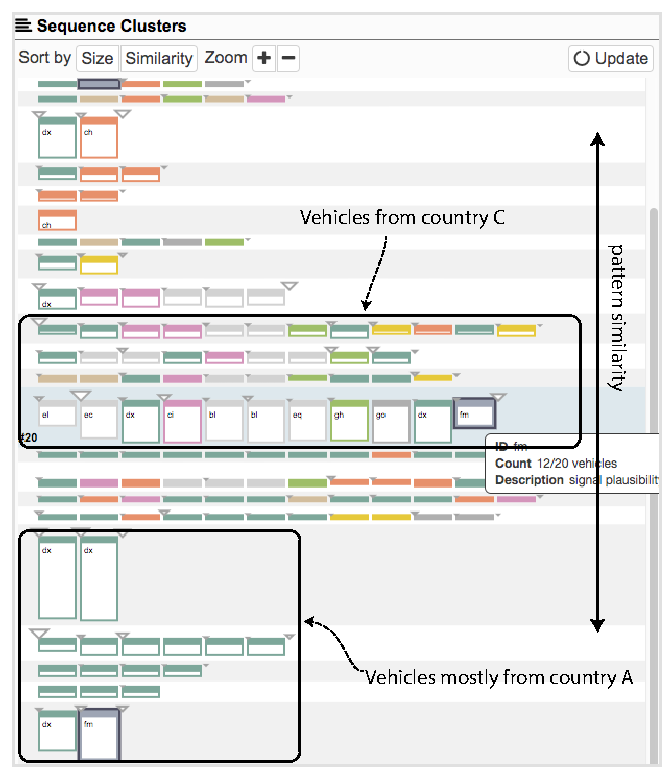
\includegraphics[width=0.96\linewidth]{pictures/case2}
	\caption{Visual summary of all sequence data. A cluster (A) with a similar pattern compared to the dominant one in Fig.~\ref{fig:teaser}. It contains vehicles sold in country C. Some other clusters (B) contain vehicles sold in country A.}
	\label{fig:case0_2}
\end{figure}

Our first usage scenario involves an expert in the automotive industry. The expert is interested in vehicle data analytics, especially analyzing the development paths of faults in vehicles. \revision{We conduct the case study together with the expert.} Today's vehicles are complex machines with interconnected modules and the faults have a significant history of development over the vehicles' lifetime. Understanding that history help with predictive diagnostics, i.e., prevent the fault from occurring or mitigate its effects in advance. Eventually this could improve the driving experience and lower the warranty cost for the car manufacturers.\looseness=-1

The fault events in vehicles are automatically recorded along with the timestamp information. We obtain a sample dataset \revision{(VFS)} from the expert. The dataset contains the fault sequences of 261 vehicles together with information such as their vehicle identification numbers(VINs), build dates and the countries they were sold to. The data is collected in one year. In total we count 154 different types of faults. The average length of the event sequence is 9.74. The maximum length is 145. Each fault also has an associated timestamp. The VIN number, the description of the events and the country names are anonymized for privacy concerns.\looseness=-1

\textbf{Data filtering.} \revision{The analyst started the analysis by filtering sequences.} Since the analyst was particularly interested in the vehicles sold to Country C, she got a subset of the data by selecting Country C in the sequence filter (Fig.~\ref{fig:teaser} (D)). The event filter shows that most of the frequently occuring faults are close to the focus event at the center (Fig.~\ref{fig:teaser} (C)). With the lasso tool, the analyst selected these events for further study. The summary view was updated to show the patterns within the filtered data. \revision{It could be observed that there is a dominant cluster with a pattern of 9 events, as highlighted in Fig.~\ref{fig:teaser} (A).}\looseness=-1

\textbf{Temporal relation exploration.} To further investigate the temporal distributions of the events in the pattern, the analyst switched the X axis in the sequences view to accurate timestamps (Fig.~\ref{fig:case0_1} (a)). By default the visualization shows the absolute time, i.e., the exact date and time of the events. To further study how the cause and effect relationship took place over time, the analyst aligned all the sequences at event \textit{gh} in the pattern (Fig.~\ref{fig:case0_1} (b)). This changed the X axis to relative time with respect to `gh'. \revision{A reference axis is shown with the movement of the mouse to indicate the time gap between the reference bar and the aligned event.} After zooming in the X axis Fig.~\ref{fig:case0_1} (c), it could be observed that the events all happened within a short time range (around 20 minutes), indicating a causal relationship that took effect pretty fast.\looseness=-1

\textbf{Detail-on-demand.} The summary view shows that quite a few events happened after the pattern ends  (Fig.~\ref{fig:teaser} (A.0)). The analyst therefore double clicked on the triangle to look into the next level-of-detail. Fig.~\ref{fig:teaser} (A.1) shows that the corrections part actually contained a large proportion of subsequences with error \textit{fm}. It could be hypothesized that \textit{fm} is also closely related to the events included in the sequential pattern, although it may not have happened yet for some of the vehicles in the cluster.\looseness=-1

\textbf{Insight validation.} Now the analyst was curious about whether vehicles sold to other countries also exhibit the same sequential fault pattern. She cleared the filtering conditions and included all the vehicles in the analysis. The summary view (Fig.~\ref{fig:case0_2}) shows the updated results and order the patterns by their similarity. The analyst observed that there is a cluster with the same sequential pattern when compared to the major cluster in Fig. 1. Hovering over the cluster also highlights the corresponding entries in the table, where the analyst observed that all the vehicles within the cluster were sold in country C. Meanwhile, the analyst also found that there is another group of clusters which contains vehicles mostly sold in country A. This observation leaded to further hypothesis about the potential root causes of these faults, such as the climate characteristics in different geographic areas or faulty parts used in producing the particular batches of cars.\looseness=-1

\subsection{Application Log Analysis for UI Design Optimization}

Our second usage scenario is application log analysis. Desktop or web applications can collect large amount of usage log data recording user interactions and many other events in the system. Log data analysis has the potential to provide important insights about users' behavioral patterns and help optimize the user interface design. \looseness=-1

We use a public dataset \revision{named Agavue} \cite{agavue}. The dataset logs the user interactions and function calls in a data visualization application in Excel. The sample dataset contains 2211 unique user sessions and 35 distinct event types. An additional preprocessing step is used to merge adjacent events of the same type. After preprocessing, the average sequence length is 11.04 and the maximum sequence length is 146.\looseness=-1

\textbf{Overview.} The analyst started with an overview of the data (Fig.~\ref{fig:case1_0}) and aligned the patterns at the \textit{appInit} event. Not surprisingly, most patterns (e.g., Fig.~\ref{fig:case1_0} (A, B)) contain a typical sequence of operations including initializing the app (\textit{appInit}, \textit{create}), resizing the window, binding data (\textit{bindFromPrompt}, \textit{readBoundData}). The analyst can click on the patterns to review the sequences in each group (Fig.~\ref{fig:case1_0} (C, D)). Pattern B represents a group of sequences with better consistency, indicated by the smaller sizes of the triangles. Pattern A represents a group of sequences that are consistent in the first few events however have more significant deviations afterwards. This observation can be easily verified by looking at the detailed views (Fig.~\ref{fig:case1_0} (C, D)).\looseness=-1

\textbf{Cause and effect relation analysis.} Since error messages popping up in an app can interrupt the users' analytic workflow and have a negative effect on user experience, it is important to understand the context in which the error messages occur and based on that, redesign the application to reduce the error messages if possible. To this end the analyst aligned the patterns at the error event (Fig.~\ref{fig:case1_1}) to study its antecedents. She observed that most errors occur after users trying to bind data to the visualization (\textit{bindFromPrompt}). One possible explanation is that the users may not be familiar with the data format requirements associated with the visualizations. This observation indicates that better interface for data binding can be designed to further improve user experience.\looseness=-1

\begin{figure*}[t]
	\centering
	\includegraphics[width=0.95\linewidth]{pictures/case4}
	\caption{The system screenshot for analyzing the Agavue dataset. Most patterns (e.g., A and B) show typical sequence of operations including initializing the app (\textit{appInit}, \textit{create}), resizing the window, binding data (\textit{bindFromPrompt}, \textit{readBoundData}, \textit{treeStats}). Pattern B represents a more homogeneous group of sequences (the triangles are quite small). Pattern A represents a group of sequences that is more similar in the first few events however has more significant deviations later.\looseness=-1
	}
	\label{fig:case1_0}
\end{figure*}









